\chapter{Diseño}

En este capítulo se abordarán las cuestiones de diseño la interfaz de usuario, explicando de manera detallada cada elemento que la compone, junto a algunos bocetos. Además, se incluirá un diagrama de navegación para saber a qué pantallas lleva cada opción.

\bigskip

Cada cuestión anteriormente mencionada se dividirá en secciones a continuación:

\section{Diseño de la Interfaz de Usuario}

La interfaz de usuario del configurador de la simulación está dividida en dos secciones principales: a la izquierda se encuentra la sección para el número de vehículos y de pilotos, la disciplina y las opciones de importación y exportación de la configuración. A la derecha está la segunda sección, compuesta por las características de cada piloto y el botón para comenzar la simulación.

\bigskip

Durante la carrera, se mostrará un listado de posiciones de los pilotos y un contador de vueltas en la parte izquierda de la pantalla. Este listado permitirá visualizar y modificar el estado de cada piloto en tiempo real. La disposición de los elementos será similar a la de disciplinas como la Fórmula 1, donde el ranking de pilotos y el contador de vueltas aparecen a la izquierda, y en cada celda de posición aparecen las tres primeras letras del apellido. En este proyecto, he decidido añadir también la primera letra del nombre, en caso de que haya varios pilotos con el mismo apellido.

\bigskip

A continuación se encuentran algunos bocetos de ambas pantallas:

\begin{figure}[H]
    \centering
    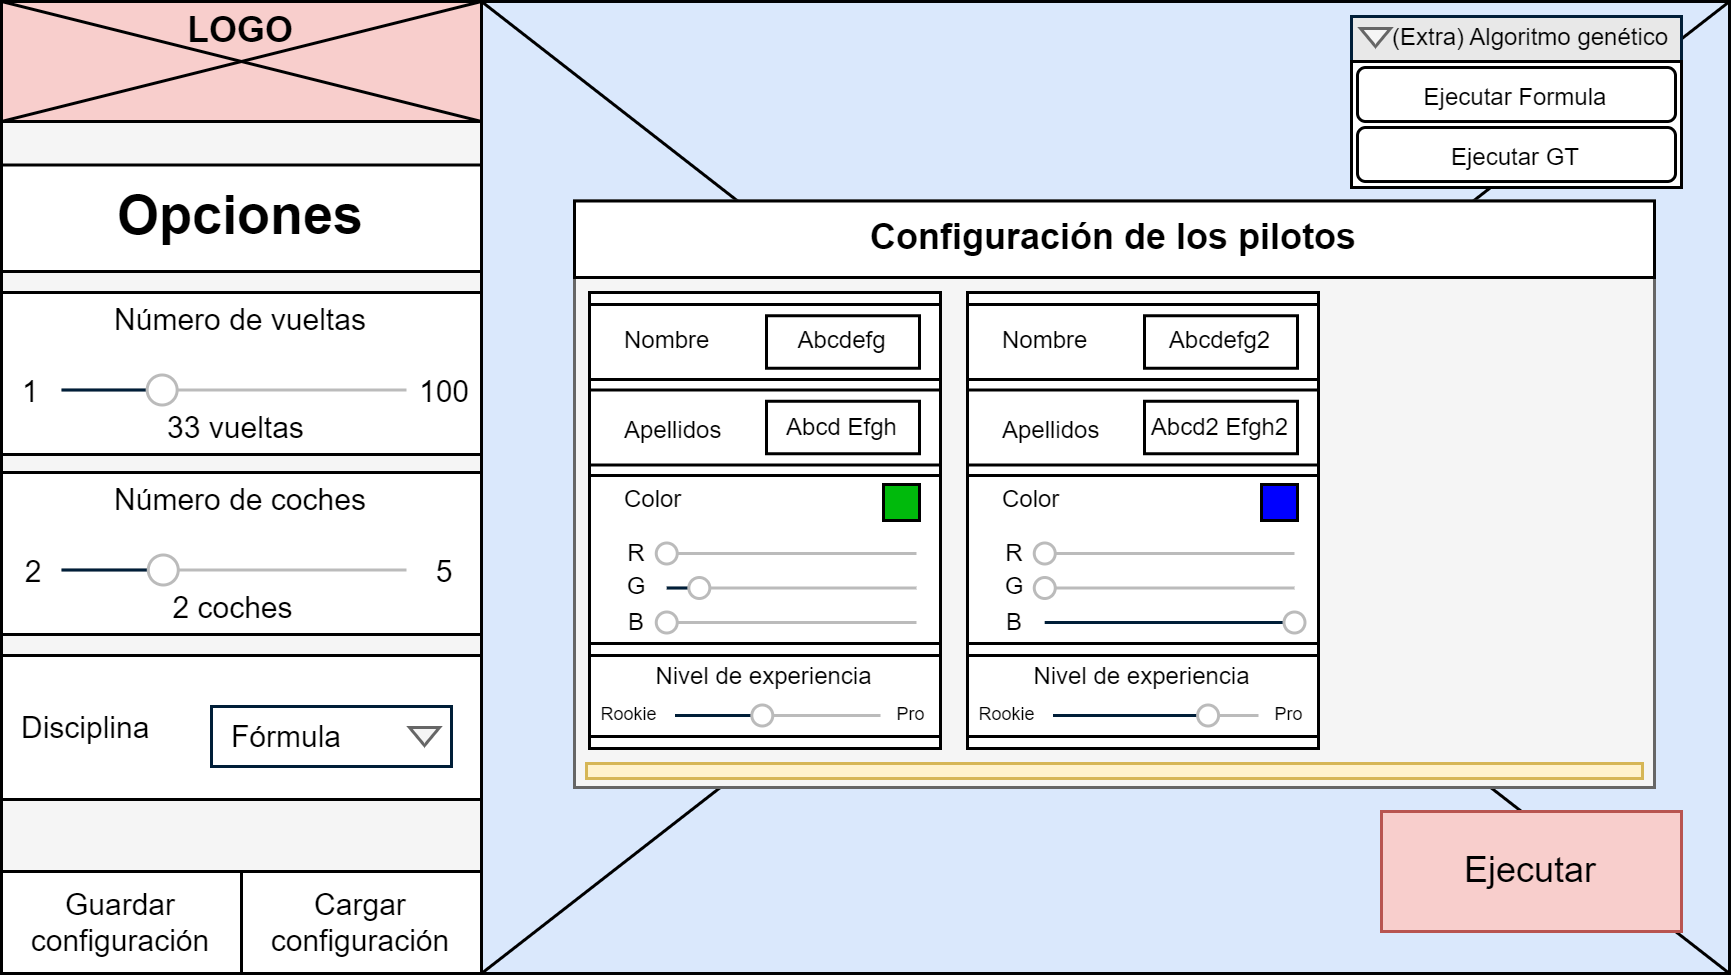
\includegraphics[width=\textwidth]{imagenes/pag1.png}
    \caption{Interfaz del configurador antes de la carrera.}
\end{figure}

\begin{figure}[H]
    \centering
    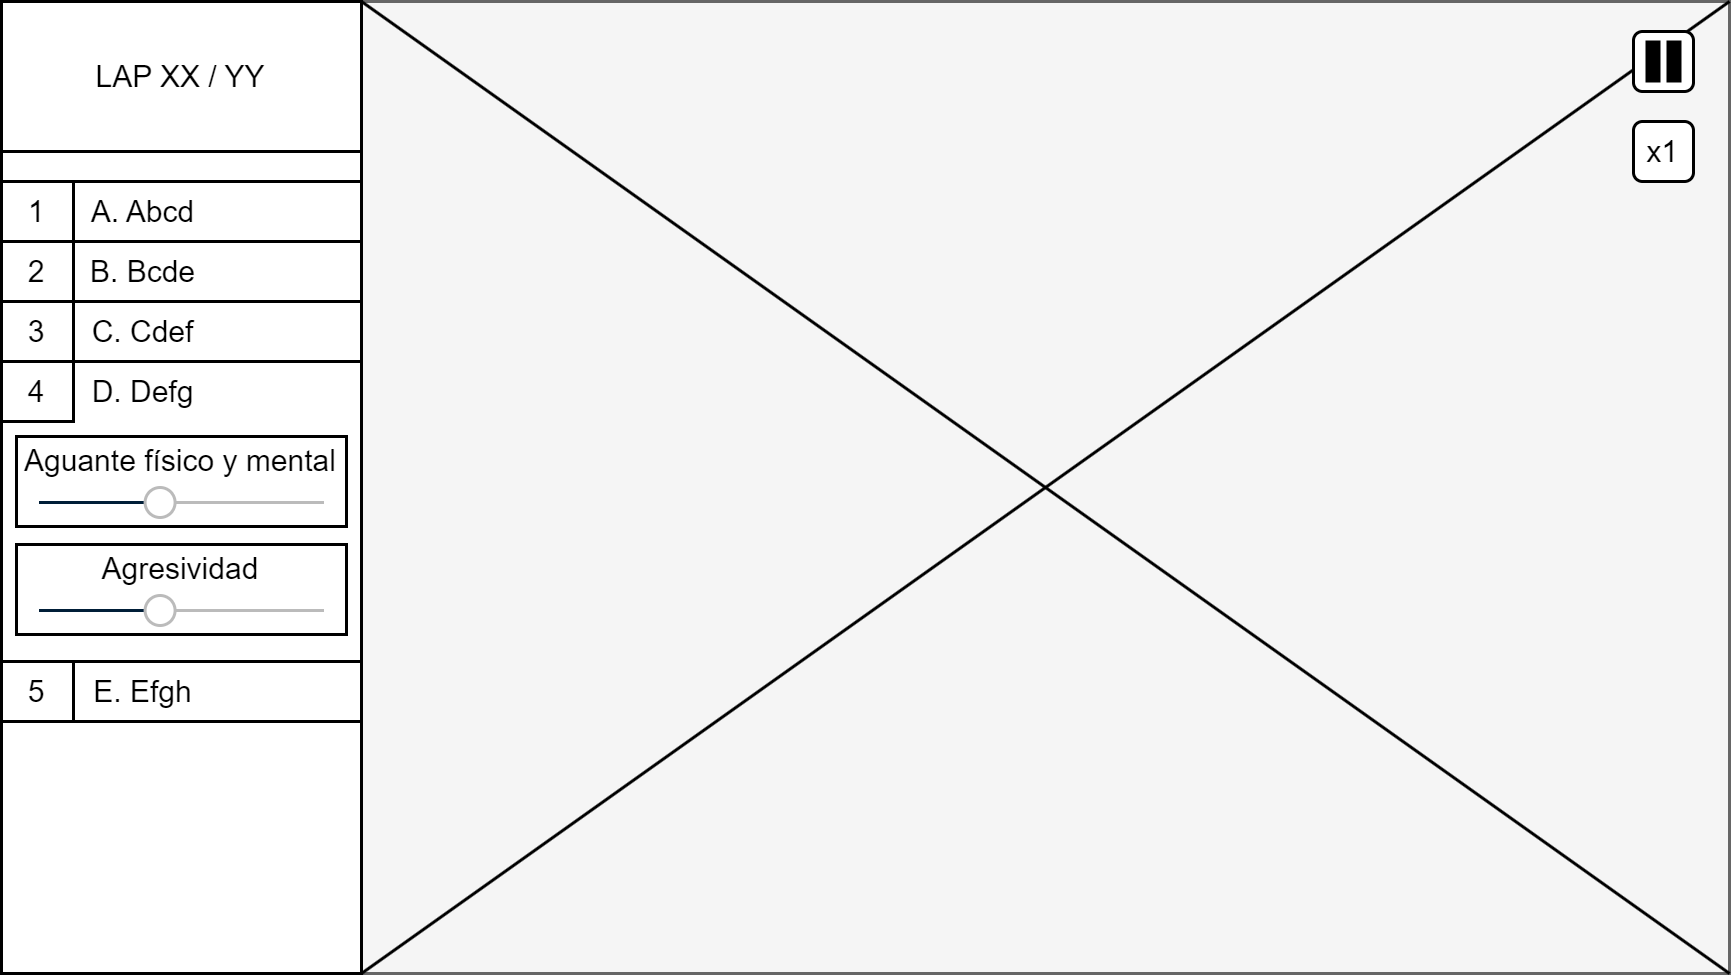
\includegraphics[width=\textwidth]{imagenes/pag2.png}
    \caption{Interfaz de las opciones durante la carrera.}
\end{figure}

\section{Diagrama de navegación}

La navegación por la interfaz de usuario en la aplicación es relativamente sencilla, al estar formada por dos pantallas: el configurador de simulación y la carrera en curso.

\bigskip
\newpage
El diagrama de navegación de la aplicación se encuentra a continuación:

% foto del diagrama de navegacion
\begin{figure}[H]
    \centering
    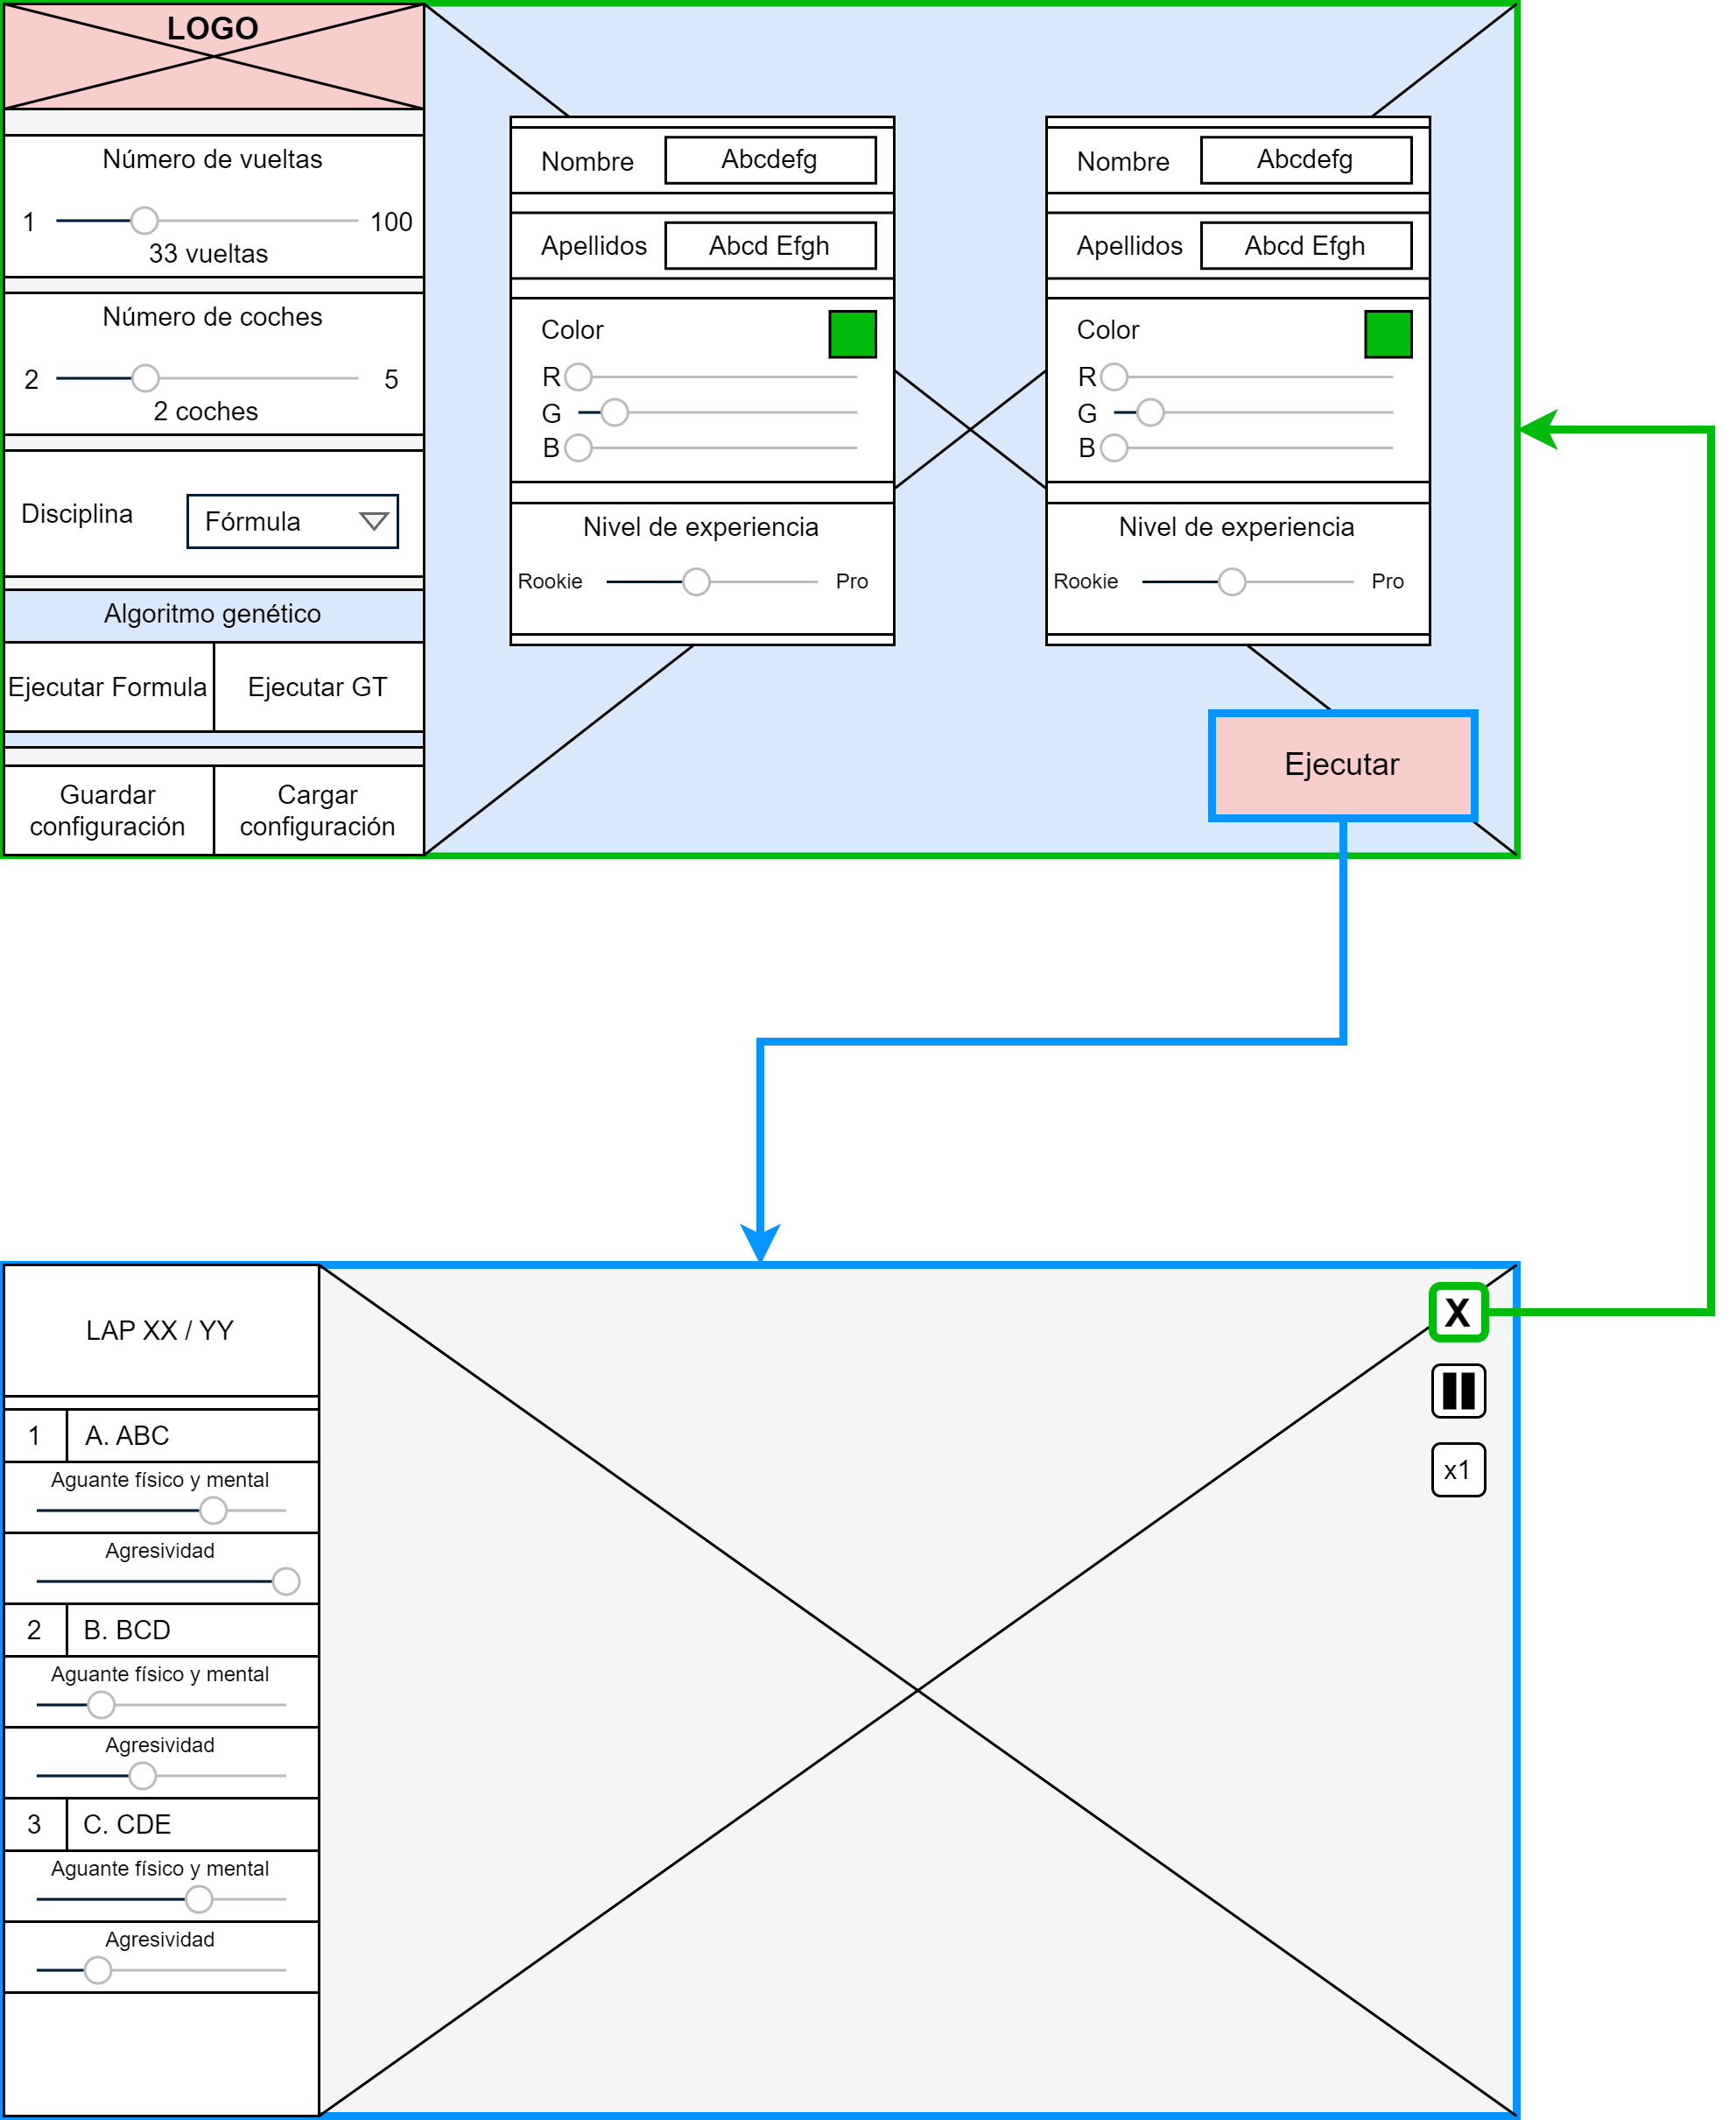
\includegraphics[width=0.9\textwidth]{imagenes/nav.png}
    \caption{Diagrama de navegación de la interfaz de usuario de la aplicación.}
 \end{figure}

Como se puede observar en el diagrama de navegación, al pulsar el botón de ejecutar aparecerá la nueva pantalla para ejecutar la simulación y dar comienzo a la carrera.

% Como se puede observar, la navegación por la aplicación es sencilla, al solo tener dos pantallas y un solo botón para ir a la siguiente. Si se pulsa sobre el botón de ejecutar en el configurador de la carrera, se procederá a cargar la simulación y dará comienzo la carrera.

\section{Entidades y atributos}

En esta sección se detallarán las distintas entidades que componen la aplicación, junto a los atributos necesarios para implementar la lógica. Cada entidad y sus atributos estarán en una subsección a continuación:

\subsection{AStarNode}
\textbf{Descripción: }Representa una celda de la matriz utilizada para ejecutar el algoritmo A*.

\bigskip

\textbf{Atributos: }
\begin{itemize}
    \item \textbf{neighbors} : AStarNode\verb|[]|
    \begin{itemize}
        \item \textbf{Descripción: }Almacena las celdas con las que colinda.
    \end{itemize}

    \item \textbf{hasObstacle} : boolean
    \begin{itemize}
        \item \textbf{Descripción: }Almacena si la celda actual está ocupada por un coche.
    \end{itemize}

    \item \textbf{isOptimal} : boolean
    \begin{itemize}
        \item \textbf{Descripción: }Indica si la celda forma parte de la ruta óptima del circuito. Puede estar ocupada.
    \end{itemize}

    \item \textbf{isDelimiter} : boolean
    \begin{itemize}
        \item \textbf{Descripción: }Indica si la celda forma parte de los límites de pista. Esta celda estará siempre ocupada y tendrá prioridad frente a las demás.
    \end{itemize}

    \item \textbf{isCheckpoint} : boolean
    \begin{itemize}
        \item \textbf{Descripción: }Indica si la celda forma parte de un checkpoint. Esta celda estará siempre libre, con independencia de si hay un coche o no.
    \end{itemize}
\end{itemize}
\subsection{AStarGrid}
\textbf{Descripción: }Representa la matriz navegación utilizada para ejecutar A*.

\bigskip

\textbf{Atributos: }
\begin{itemize}
    \item \textbf{nodes} : AStarNode\verb|[]|
    \begin{itemize}
        \item \textbf{Descripción: }Almacena todos los nodos que forman la malla de navegación. El primero es el de más arriba a la izquierda y el último es el de más abajo a la derecha.
    \end{itemize}
    \item \textbf{gridSize} : Integer
    \begin{itemize}
        \item \textbf{Descripción: }Cantidad de cubos que va a haber a lo largo y a lo ancho.
    \end{itemize}
    \item \textbf{nodeSize} : Integer
    \begin{itemize}
        \item \textbf{Descripción: }Tamaño que tendrá la celda. Por defecto es 100.
    \end{itemize}
    \item \textbf{startingPosition} : Vector
    \begin{itemize}
        \item \textbf{Descripción: }Posición por la que se debe comenzar a generar la malla. Esta coordenada representa la posición más a la izquierda y arriba de la malla.
    \end{itemize}
    % \item \textbf{openList} : PriorityQueue
\end{itemize}

\subsection{PriorityQueue}
\textbf{Descripción: }Representa una cola con prioridad ascendente, utilizada para A*.

\bigskip

\textbf{Atributos: }
\begin{itemize}
    \item \textbf{queue} : QueueElement\verb|[]|
    \begin{itemize}
        \item \textbf{Descripción: }Lista con todos los nodos visitados y sus costes. Se encuentran ordenados.
    \end{itemize}
\end{itemize}


\subsection{QueueElement}
\textbf{Descripción: }Estructura de datos que es utilizada por PriorityQueue para realizar los cálculos.

\bigskip

\textbf{Atributos: }
\begin{itemize}
    \item \textbf{node} : AStarNode
    \begin{itemize}
        \item \textbf{Descripción: }Representa el nodo que se va a insertar en la cola.
    \end{itemize}

    \item \textbf{cost} : Float
    \begin{itemize}
        \item \textbf{Descripción: }Representa el coste total del nodo, incluyendo la heurística.
    \end{itemize}
\end{itemize}
\subsection{AStarPathfinder}
\textbf{Descripción: }Implementa el algoritmo A* para ser utilizado por los coches.


\subsection{SportsCarPawn\_AI}
\textbf{Descripción: }Representa a los coches que compiten por el circuito.

\subsection{Marcador}
\textbf{Descripción: }Entidad utilizada para generar la lista de posiciones y el contador de vueltas, así como la actualización de ambos.

\bigskip

\textbf{Atributos: }
\begin{itemize}
    \item \textbf{uiRef} : Panel
    \begin{itemize}
        \item \textbf{Descripción: }Referencia al panel con el contador de vueltas y el ranking.
    \end{itemize}
    
    \item \textbf{cars} : SportsCarPawn\_AI\verb|[]|
    \begin{itemize}
        \item \textbf{Descripción: }Almacena una referencia de todos los coches de la carrera. Se encuentran siempre ordenados, estando en posiciones menores los vehículos que mejor van.
    \end{itemize}

    \item \textbf{checkpoints} : Checkpoint\verb|[]|
    \begin{itemize}
        \item \textbf{Descripción: }Almacena todos los checkpoints que hay en la escena. Están ordenados de manera ascendente, de forma que los índices superiores indican checkpoints posteriores del circuito.
    \end{itemize}

    \item \textbf{currentLap} : Integer
    \begin{itemize}
        \item \textbf{Descripción: }Almacena la vuelta actual de la carrera.
    \end{itemize}

    \item \textbf{MAX\_LAPS} : Integer 
    \begin{itemize}
        \item \textbf{Descripción: }Indica el número de vueltas que tiene la carrera.
    \end{itemize}
\end{itemize}

\subsection{Panel}
\textbf{Descripción: }Interfaz de usuario en la que se muestra el contador de vueltas y el ranking.

\bigskip

\textbf{Atributos: }
\begin{itemize}
    \item \textbf{LAPS} : Text Widget
    \begin{itemize}
        \item \textbf{Descripción: }Es el texto que aparece en la propia interfaz de usuario.
    \end{itemize}

    \item \textbf{VerticalBox\_0} : Vertical Box
    \begin{itemize}
        \item \textbf{Descripción: }Marco donde se almacena cada celda de la clase Posicion con la información de cada piloto.
    \end{itemize}
    % \item cars
\end{itemize}

\subsection{Posicion}
\textbf{Descripción: }Cuadro básico que representa una celda en el ranking.

\bigskip

\textbf{Atributos: }
\begin{itemize}
    \item \textbf{Agresividad} : Sliding Bar
    \begin{itemize}
        \item \textbf{Descripción: }Barra deslizadora que indica la agresividad del conductor.
    \end{itemize}

    \item \textbf{Aguante} : Sliding Bar
    \begin{itemize}
        \item \textbf{Descripción: }Barra deslizadora que indica el aguante físico y mental del conductor.
    \end{itemize}

    % \item TextBlock_47
\end{itemize}

\subsection{ArrayOfCars}
\textbf{Descripción: }Estructura utilizada para almacenar el número de coches que hay en un checkpoint concreto.

\bigskip

\textbf{Atributos: }
\begin{itemize}
    \item \textbf{cars} : SportsCarPawn\_AI\verb|[]|
    \begin{itemize}
        \item \textbf{Descripción: }Almacena todos los coches para un checkpoint dado.
    \end{itemize}
\end{itemize}

\subsection{ArrayOfArrayOfCars}
\textbf{Descripción: }Estructura que almacena en que vuelta y en que checkpoint se encuentra cada vehículo.

\bigskip

\textbf{Atributos: }
\begin{itemize}
    \item \textbf{laps} : Map<Integer, ArrayOfCars>
    \begin{itemize}
        \item \textbf{Descripción: }Almacena todos los coches y sus checkpoints que se encuentran en una vuelta dada.
    \end{itemize}
\end{itemize}


\subsection{PID}
\textbf{Descripción: }Entidad encargada de implementar la lógica del PID, exponiendo funciones para su uso.

\bigskip

\textbf{Atributos: }
\begin{itemize}
    \item \textbf{Kp} : Float
    \begin{itemize}
        \item \textbf{Descripción: }Constante proporcional del PID.
    \end{itemize}
    
    \item \textbf{Ki} : Float
    \begin{itemize}
        \item \textbf{Descripción: }Constante integral del PID.
    \end{itemize}
    
    \item \textbf{Kd} : Float
    \begin{itemize}
        \item \textbf{Descripción: }Constante derivativa del PID.
    \end{itemize}        

    % \item minoutput, maxoutput, erroractualfuera

    \item \textbf{errorPasado} : Float
    \begin{itemize}
        \item \textbf{Descripción: }Error en el instante anterior al actual. Necesario para implementar la componente integral.
    \end{itemize}

    \item \textbf{errorAcumulado} : Float
    \begin{itemize}
        \item \textbf{Descripción: }Error acumulado con el tiempo. Esta variable es utilizada por la componente integral.
    \end{itemize}
\end{itemize}

\subsection{Checkpoint}
\textbf{Descripción: }Entidad encargada de poner un checkpoint en el mundo, para poder realizar cálculos.

\bigskip

\textbf{Atributos: }
\begin{itemize}
    \item \textbf{id} : Integer
    \begin{itemize}
        \item \textbf{Descripción: }Identificador del checkpoint. Este valor debe ir creciendo en el mismo orden en el que los coches pasan los checkpoints en el circuito.
    \end{itemize}
    
    \item \textbf{speed} : Float
    \begin{itemize}
        \item \textbf{Descripción: }Velocidad aconsejable a la que debe pasar el coche el tramo hasta el siguiente checkpoint.
    \end{itemize}

    % \item \textbf{apexType}
\end{itemize}

\subsection{SplinePath}
\textbf{Descripción: }Entidad que almacena un spline.

\subsection{ChangeSpline}
\textbf{Descripción: }Entidad referente al algoritmo genético. Utilizada para cambiar de spline prefijado en el modo entrenamiento.

\subsection{Genome}
\textbf{Descripción: }Estructura de datos que almacena las constantes del PID de un coche, así como su identificador y \textit{fitness} para el algoritmo genético.

\bigskip

\textbf{Atributos: }
\begin{itemize}
    \item \textbf{Kp} : Float
    \begin{itemize}
        \item \textbf{Descripción: }Constante proporcional del PID.
    \end{itemize}
    
    \item \textbf{Ki} : Float
    \begin{itemize}
        \item \textbf{Descripción: }Constante integral del PID.
    \end{itemize}    

    \item \textbf{Kd} : Float
    \begin{itemize}
        \item \textbf{Descripción: }Constante derivativa del PID.
    \end{itemize}    

    \item \textbf{fitness} : Float
    \begin{itemize}
        \item \textbf{Descripción: }Almacena la probabilidad de ser escogido para la siguiente generación.
    \end{itemize}

    \item \textbf{id} : Integer
    \begin{itemize}
        \item \textbf{Descripción: }Almacena el identificador del vehículo.
    \end{itemize}
\end{itemize}

\subsection{TrainingStop}
\textbf{Descripción: }Utilizado en el algoritmo genético. Marca el punto final de los coches.

\bigskip

\textbf{Atributos: }
\begin{itemize}
    \item \textbf{currentCars} : Integer
    \begin{itemize}
        \item \textbf{Descripción: }Almacena el número de vehículos que aún siguen en pie. Esto es debido a que aquellos coches que se chocan o se caen son eliminados.
    \end{itemize}

    \item \textbf{MAX\_GENOMES} : Integer
    \begin{itemize}
        \item \textbf{Descripción: }Indica el número de coches que se lanzan por generación.
    \end{itemize}

    \item \textbf{values} : genome\verb|[]|
    \begin{itemize}
        \item \textbf{Descripción: }Almacena todas las constantes de los hijos de una generación.
    \end{itemize}

    \item \textbf{identificadores} : Integer
    \begin{itemize}
        \item \textbf{Descripción: }Contador para asignar el identificador a todos los coches.
    \end{itemize}

    \item \textbf{probabilidadMutacion} : Float
    \begin{itemize}
        \item \textbf{Descripción: }Indica la probabilidad con la que un coche pueda llegar a tener una mutación.
    \end{itemize}

    % isEnabled (hay que eliminarlo en el proyecto final), prueba
\end{itemize}